\documentclass[journal]{./IEEE/IEEEtran}
\usepackage{cite,graphicx}
\usepackage{multirow}

\newcommand{\SPTITLE}{Master-Slave Distributed Z-Score Normalization of a Square Matrix using Socket Communication with Multi-threading and CPU Affinity}
\newcommand{\ADVISEE}{Jadon C. Sacayanan}
% \newcommand{\ADVISER}{Adviser M. Name}

\newcommand{\BSCS}{Bachelor of Science in Computer Science}
\newcommand{\ICS}{Institute of Computer Science}
\newcommand{\UPLB}{University of the Philippines Los Ba\~{n}os}
\newcommand{\REMARK}{\thanks{Presented to the Faculty of the \ICS, \UPLB\
                             in partial fulfillment of the requirements
                             for the Degree of \BSCS}}
        
\markboth{CMSC 180 Introduction to Parallel Computing, \ICS}{}
\title{\SPTITLE}
% \author{\ADVISEE~and~\ADVISER%
\author{\ADVISEE
\REMARK
}
\pubid{\copyright~2025~ICS \UPLB}

%%%%%%%%%%%%%%%%%%%%%%%%%%%%%%%%%%%%%%%%%%%%%%%%%%%%%%%%%%%%%%%%%%%%%%%%%%

\begin{document}

% TITLE
\maketitle

% ABSTRACT
\begin{abstract}
    This research examines the performance of a multi-threaded master-slave architecture for computing the Z-score normalization of a square matrix. The program utilizes socket communication to distribute submatrices to multiple slave processes, allowing for parallel processing. The study investigates the impact of varying the number of slave processes on the runtime of the Z-score normalization computation. The results demonstrate that increasing the number of slaves significantly reduces runtime, highlighting the benefits of distributed computing for large-scale matrix computations.
\end{abstract}

% INDEX TERMS
\begin{keywords}
parallel computing, multi-threading, CPU affinity, Z-score normalization, matrix computation
\end{keywords}

% INTRODUCTION
\section{Introduction}
Efficient data processing is crucial in high-performance computing, where optimizing computational tasks can significantly improve execution speed. When managing large datasets, data can be distributed to enable parallel processing, which may reduce processing time and improve overall performance.

\subsection{Z-score normalization}
The Z-score indicates how far a value deviates from the mean, measured in standard deviations, ensuring that all measurements are on the same scale\cite{andrade2021z}.
All distributions expressed in Z-scores have the same mean (0) and the same variance (1). This allows Z-scores to be used in comparing observations coming from different distributions \cite{abdi2007z}.
To compute for the Z-score, we use the formula:
\begin{equation}
\label{zscoreformula}
    z=\frac{x-\mu}{\sigma}
\end{equation}
where:
\( x \) is the observed value,  
\( \mu \) is the mean, and
\( c \) is the standard deviation.

In columnar Z-score normalization, each column in a matrix is normalized independently by applying the Z-score formula to every value.
For each column, the mean and standard deviation are computed separately, and each value is transformed by subtracting the column's mean and dividing by its standard deviation.
Since Z-scores standardize measurements to the same scale by effectively removing units, they allow for the comparison of values that were originally measured in different units \cite{abdi2007z}.

\subsection{Distributed computing}
Distributed computing refers to programs that make calls to other address spaces, which may reside on the same machine or potentially on remote machines. This includes technologies such as remote object invocation, where tasks are distributed across different systems, allowing for the execution of processes on separate nodes and facilitating efficient resource utilization in a networked environment
\cite{waldo1996note}.

\subsection{Socket programming}
Socket programming is a way of connecting two nodes on a network to communicate with each other. One socket(node) listens on a particular port at an IP, while the other socket reaches out to the other to form a connection. The server forms the listener socket while the client reaches out to the server \cite{socketc}.

\subsection{Thread}
A thread is an abstract entity that represents the execution of a sequence of instructions within a program.
It is a lightweight component consisting of essential elements like registers, a stack, and other associated data.
A thread is the smallest unit of execution, capable of being scheduled and executed independently on a CPU.
Each thread can run independently, allowing multiple threads to execute in parallel, thereby improving the efficiency of the program \cite{lewis1996pthreads}.

\subsection{CPU affinity}
CPU affinity is a technique that binds a thread or process to a specific CPU core, preventing the operating system from migrating it to another core.
CPU affinity is optimizing cache performance.
When a thread is bound to a specific core, it can take advantage of the cache's contents, reducing cache misses and improving performance \cite{love2003kernel}.


\subsection{Cache awareness}
When the processor needs to access data, it first checks its cache.
If the data is found in the cache, it is called a cache hit, allowing for fast retrieval.
However, if the data is not present, a cache miss occurs, requiring the processor to fetch the data from main memory, which is significantly slower.

The processor does not work by retrieving a single byte of data, but instead fetches a larger block of memory called a cache line.
By loading an entire cache line at once, the processor increases the likelihood that future memory accesses will be served from the cache rather than requiring additional slow memory fetches.
This reduces the frequency of cache misses and enhances overall processing efficiency \cite{newhehe}.

\subsection{Temporal locality}
Programs has the tendency to repeatedly use the same data items during their execution. This principle is the basis for caching and suggests that it is beneficial to store frequently accessed instructions or data items nearby for future use \cite{jacob2010memory}.


% OBJECTIVES
\section{Objectives}
    This research activity aims to analyze the performance and efficiency of distributing matrix computations across multiple processes using socket communication.
    Specifically, it aims to:
\begin{enumerate}
    \item Implement a master-slave architecture that distributes submatrices to multiple processes via socket communication.
    \item Solve the Z-score normalization problem using the master-slave architecture.
    \item Investigate the impact of varying the number of slave processes (t) on solving the Z-score normalization problem.
\end{enumerate}


% MATERIALS AND METHODS
\section{Materials and Methods}
A program was developed to distribute parts of an n x n matrix from a master to multiple slave machines using sockets. For each matrix size n, the distribution process was executed three times to calculate the average runtime. To ensure accurate measurements, all tests were conducted under controlled conditions with no other applications running, minimizing external influences on network and system performance.


\subsection{The program}
The program is written in C and begins by prompting the user to input three values: n, the size of the square matrix; p, the port number used for socket communication; and s, a value that determines the role of the program, where 0 indicates a master and 1 indicates a slave. These inputs define how the program will behave during the matrix distribution process.



\subsection{Master}
When the program is run as a master, it generates an n × n random square matrix. The matrix is then divided into submatrices, each with n columns and approximately n/t rows, where t is the number of slaves. If n is not exactly divisible by t, the remaining rows are distributed among the first few slaves, with each receiving at most one additional row. Rather than creating separate matrices, the master identifies the start and end row indices for each submatrix, referencing the original matrix directly.

Once all submatrices are determined, the master establishes socket connections to the slave machines. It then sends each submatrix, number by number, to its assigned slave. After transmission, the master waits for the computed Z-scores from the slaves. Each slave sends back the computed Z-scores, which are then stored in a dynamically allocated array. The master waits for all slaves to finish before closing the socket connections.

Each connection to a slave is handled by a separate thread, allowing the master to manage multiple connections concurrently. This allows the master to send submatrices to multiple slaves simultaneously. At the same time, the each thread only waits for a particular slave to finish computation while other threads continue to send submatrices to other slaves. This design improves the overall efficiency of the program by reducing idle time during communication. This would also mean that the only idle time of the master is when it is waiting for the last slave to finish computation.

Excess computations are avoided by using the same array for both sending and receiving data. This means that no temporary matrices are created, and the original matrix is modified in place. 

The master also measures the time taken for the entire process, from establishing connections to receiving the final Z-scores. This time measurement is done using the sys/time.h header, capturing timestamps before and after the socket communication.

\subsection{Slave}
When the program is run as a slave, it waits for a connection from the master. Upon connection, the slave receives the submatrix data, transmitted number by number, and stores it in a dynamically allocated array sized according to the expected number of rows and columns. After successfully receiving the entire submatrix, the slave computes the Z-scores for each element in the submatrix using the formula provided in Equation \ref{zscoreformula}. The computed Z-scores are then sent back to the master, and the socket connection is closed.

The slave also measures the time taken for the computation process only and does not include the socket communication time. This is done by capturing timestamps before and after the computation phase, allowing for a clear understanding of the time spent on the actual Z-score calculations.

The computation of the Z-score normalization is done in a parallel. The submatrix is divided into t parts, and each part is assigned to a separate thread. Each thread computes the Z-scores for its assigned part of the submatrix independently, allowing for concurrent processing and improved performance.

Just like the master, the slave uses the same array for both sending and receiving data. This means that no temporary matrices are created, and the original matrix is modified in place.

\subsection{Threading}
The program uses the pthread library to create threads. In both the master and slave roles, each thread is responsible for handling a single socket connection, starting from establishing the connection (sending or listening) until the communication is closed. This design allows concurrent handling of multiple connections, enabling parallel distribution and reception of submatrices.

\subsection{CPU affinity}
The program determines the number of available cores using the sysconf function and assigns each thread to a specific core using the CPU affinity feature. To ensure system stability and prevent resource contention, one core is reserved for main system processes, such as the operating system scheduler, background services, and essential system tasks. Each thread is pinned to a dedicated CPU core using the CPU set function, preventing the operating system from migrating threads between cores and reducing interference from other system functions. This avoids the overhead of thread migration and maximizes program performance.

\subsection{Computing for the columnar Z-score normalization}
To compute the z-score normalization of a two-dimensional matrix, a loop traverses across the columns of the matrix.

In each column, a loop computes the mean by taking the sum of all elements in the column and dividing the result by the height of the column.
The standard deviation is also computed using a loop by taking the square root of the sum of the squared differences between each element and the mean, divided by the height of the column.

Finally, the z-score for each element is calculated using Formula \ref{zscoreformula} and directly stored in the same array.
No temporary matrices are created since the original matrix is modified in place with the help of pointers.

These computations are done by each individual thread on the submatrix assigned to it.


\subsection{Time measurement}
The program uses the sys/time.h header to measure execution time by capturing a timestamp with gettimeofday() immediately before establishing a connection. A second timestamp is recorded after the socket is closed. The elapsed time is then calculated by determining the difference between these two timestamps. This time measurement only includes the communication phase and does not account for the preparation of the threads, such as setting up their arguments.


\subsection{Distributed computing}
The program utilizes four machines, running up to four instances of the slave program on each machine. Different configurations were used depending on the value of n. For n=2, two machines were used, each running one instance of the slave. For n=4, four machines were used with one instance of the slave on each. For n=8, the same four machines were used, each running two instances of the slave. Finally, for n=16, all four machines ran four instances of the slave each.

It also utilized a personalized one-to-many broadcast mechanism, where the master node efficiently sends data to multiple slave nodes simultaneously. This approach minimizes communication overhead by leveraging non-blocking socket operations, ensuring that the master can continue transmitting data to other nodes without waiting for acknowledgments from previously contacted nodes.


\subsection{System information}
The program was executed on an Acer desktop equipped with an Intel® Core™ i5-13400 processor and 16GB of memory, running Ubuntu 22.04.5 LTS. Both the master and all slave machines used the same hardware and software configuration.

% RESULTS AND DISCUSSION
\section{Results and Discussion}
The program was executed independently for three iterations where each iteration was run with different values of n and t. The average runtime was calculated for each configuration, and the results were recorded.

% Please add the following required packages to your document preamble:
% \usepackage{multirow}
% Please add the following required packages to your document preamble:
% \usepackage{multirow}

\subsection{Runtime results of the master process}

The master process measures the time elapsed from the start of the socket communication until the last Z-score is received. The results are shown in Table \ref{master} and Figure \ref{multi_chart}. The average runtime is calculated by taking the mean of the three runs for each configuration.

\begin{table}[]
\begin{center}
    \caption{Time elapsed as reported by the master process.}
    \begin{tabular}{|c|c|ccc|c|}
\hline
\multirow{2}{*}{\textbf{n}} & \multirow{2}{*}{\textbf{t}} & \multicolumn{3}{c|}{\textbf{Time Elapsed (seconds)}} & \multirow{2}{*}{\textbf{\begin{tabular}[c]{@{}c@{}}Average\\ Runtime\end{tabular}}} \\ \cline{3-5}
 &  & \multicolumn{1}{c|}{\textbf{Run 1}} & \multicolumn{1}{c|}{\textbf{Run 2}} & \textbf{Run 3} &  \\ \hline
20000 & 2 & \multicolumn{1}{c|}{78.598209} & \multicolumn{1}{c|}{78.493001} & 78.527834 & 78.539681 \\ \hline
20000 & 4 & \multicolumn{1}{c|}{64.100006} & \multicolumn{1}{c|}{64.215567} & 64.178477 & 64.164683 \\ \hline
20000 & 8 & \multicolumn{1}{c|}{55.113805} & \multicolumn{1}{c|}{55.858100} & 55.167691 & 55.379865 \\ \hline
20000 & 16 & \multicolumn{1}{c|}{55.203650} & \multicolumn{1}{c|}{55.435277} & 55.194854 & 55.277927 \\ \hline
25000 & 2 & \multicolumn{1}{c|}{122.330935} & \multicolumn{1}{c|}{122.325718} & 122.334482 & 122.330378 \\ \hline
25000 & 4 & \multicolumn{1}{c|}{100.327608} & \multicolumn{1}{c|}{100.423944} & 100.273722 & 100.341758 \\ \hline
25000 & 8 & \multicolumn{1}{c|}{86.651681} & \multicolumn{1}{c|}{86.035480} & 86.535978 & 86.407713 \\ \hline
25000 & 16 & \multicolumn{1}{c|}{85.911332} & \multicolumn{1}{c|}{85.554153} & 86.145068 & 85.870184 \\ \hline
30000 & 2 & \multicolumn{1}{c|}{178.102334} & \multicolumn{1}{c|}{178.096227} & 178.109482 & 178.102681 \\ \hline
30000 & 4 & \multicolumn{1}{c|}{144.105122} & \multicolumn{1}{c|}{144.169503} & 144.517692 & 144.264106 \\ \hline
30000 & 8 & \multicolumn{1}{c|}{124.863588} & \multicolumn{1}{c|}{124.026440} & 124.240050 & 124.376693 \\ \hline
30000 & 16 & \multicolumn{1}{c|}{124.139228} & \multicolumn{1}{c|}{124.010230} & 123.914170 & 124.021209 \\ \hline
    \end{tabular}
    \label{master}
\end{center}
\end{table}

\begin{figure}
    \centering
    \fbox{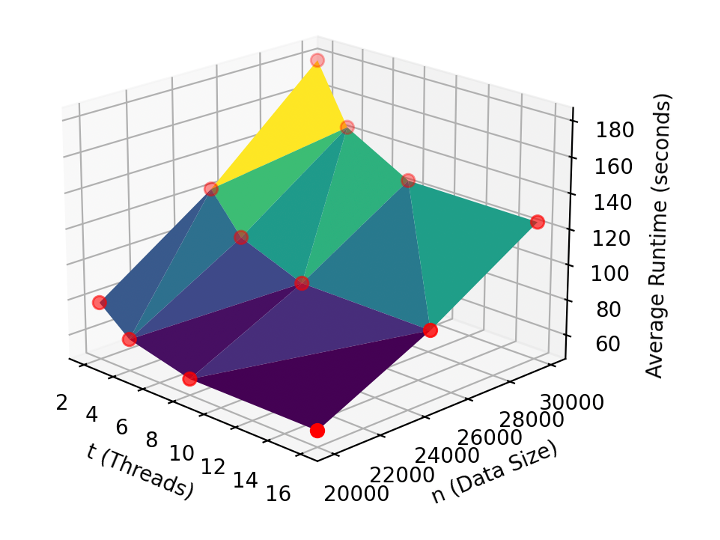
\includegraphics[width=0.45\textwidth]{images/plot_master.png}}
    \caption{Runtime Trends over Data Size and Threads for the Master Process}
    \label{plot_master}
\end{figure}

Table \ref{master} shows that lower the fastest average runtime is achieved at n=20000 and t=16, with an average runtime of 55.277927 seconds. The slowest average runtime is at n=30000 and t=2, with an average runtime of 178.102681 seconds.

As visualized in Figure \ref{plot_master}, the average runtime decreases as the number of slaves increases, indicating that distributing the workload across multiple slaves improves performance. The trend is consistent across different matrix sizes, with larger matrices shows more pronounced improvements in runtime as the number of slaves increases. 

Figure \ref{plot_master} also shows that the average runtime increases as the matrix size increases. This is expected, as larger matrices require more computations and data transfer, leading to longer processing times.

Overall, the results indicate that the average runtime decreases at lower matrix sizes with an increased number of slaves.

\subsection{Runtime results of the slave process}
The slave process measures the time elapsed for the computation of the Z-scores only. The maximum computation time accross the different slaves is recorded. The results are shown in Table \ref{slave} and Figure \ref{plot_slave}. The average runtime is calculated by taking the mean of the three runs for each configuration.

\begin{table}[]
\begin{center}
    \caption{Time elapsed as reported by the slave processes.}
    \begin{tabular}{|c|c|ccc|c|}
\hline
\multirow{2}{*}{\textbf{n}} & \multirow{2}{*}{\textbf{t}} & \multicolumn{3}{c|}{\textbf{Max Time Elapsed (seconds)}} & \multirow{2}{*}{\textbf{\begin{tabular}[c]{@{}c@{}}Average\\ Runtime\end{tabular}}} \\ \cline{3-5}
 &  & \multicolumn{1}{c|}{\textbf{Run 1}} & \multicolumn{1}{c|}{\textbf{Run 2}} & \textbf{Run 3} &  \\ \hline
20000 & 2 & \multicolumn{1}{c|}{0.569854} & \multicolumn{1}{c|}{0.585570} & 0.576342 & 0.577255 \\ \hline
20000 & 4 & \multicolumn{1}{c|}{0.294665} & \multicolumn{1}{c|}{0.301091} & 0.294198 & 0.296651 \\ \hline
20000 & 8 & \multicolumn{1}{c|}{0.292461} & \multicolumn{1}{c|}{0.294098} & 0.293862 & 0.293474 \\ \hline
20000 & 16 & \multicolumn{1}{c|}{0.290630} & \multicolumn{1}{c|}{0.292355} & 0.288578 & 0.290521 \\ \hline
25000 & 2 & \multicolumn{1}{c|}{0.920307} & \multicolumn{1}{c|}{0.918204} & 0.922745 & 0.920419 \\ \hline
25000 & 4 & \multicolumn{1}{c|}{0.549026} & \multicolumn{1}{c|}{0.462104} & 0.458852 & 0.489994 \\ \hline
25000 & 8 & \multicolumn{1}{c|}{0.458849} & \multicolumn{1}{c|}{0.486524} & 0.467496 & 0.470956 \\ \hline
25000 & 16 & \multicolumn{1}{c|}{0.438729} & \multicolumn{1}{c|}{0.450675} & 0.462885 & 0.450763 \\ \hline
30000 & 2 & \multicolumn{1}{c|}{1.324466} & \multicolumn{1}{c|}{1.321009} & 1.328112 & 1.324529 \\ \hline
30000 & 4 & \multicolumn{1}{c|}{0.663461} & \multicolumn{1}{c|}{0.666165} & 0.648713 & 0.659446 \\ \hline
30000 & 8 & \multicolumn{1}{c|}{0.659471} & \multicolumn{1}{c|}{0.655963} & 0.652604 & 0.656013 \\ \hline
30000 & 16 & \multicolumn{1}{c|}{0.641995} & \multicolumn{1}{c|}{0.659937} & 0.652261 & 0.651398 \\ \hline
    \end{tabular}
    \label{slave}
\end{center}
\end{table}

\begin{figure}
    \centering
    \fbox{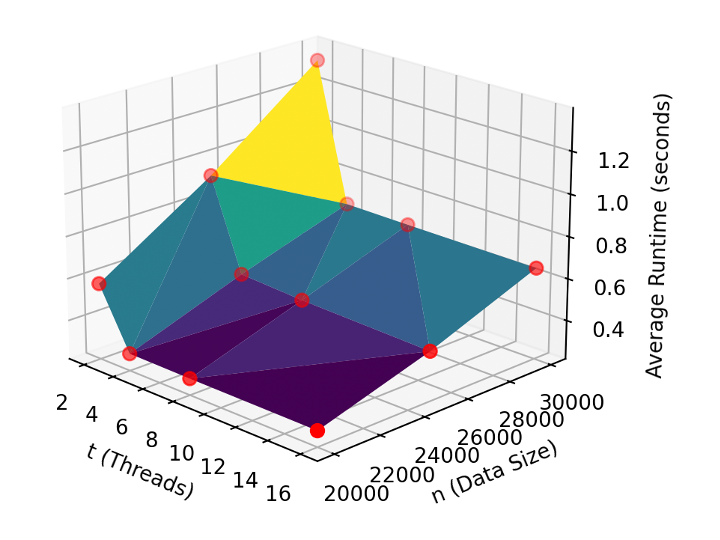
\includegraphics[width=0.45\textwidth]{images/plot_slave.png}}
    \caption{Runtime Trends over Data Size and Threads for the Slave Processes}
    \label{plot_slave}
\end{figure}

Table \ref{slave} shows that the fastest average runtime is achieved at n=20000 and t=16, with an average runtime of 0.290521 seconds. The slowest average runtime is at n=30000 and t=2, with an average runtime of 1.324529 seconds.

As visualized in Figure \ref{plot_slave}, the average runtime decreases as the number of slaves increases, indicating that distributing the workload across multiple slaves improves performance. The trend is consistent across different matrix sizes, with larger matrices shows more pronounced improvements in runtime as the number of slaves increases.

Figure \ref{plot_slave} also shows that the average runtime increases as the matrix size increases. This is expected, as larger matrices require more computations and data transfer, leading to longer processing times.

Overall, the results indicate that the average runtime decreases at lower matrix sizes with an increased number of slaves.

\subsection{Performance metrics}

\begin{table}[]
\begin{center}
    \caption{Performance metrics of the parallel, distributed Pearson Correlation Coefficient}
    \begin{tabular}{|c|c|c|cccc|}
\hline
\multirow{2}{*}{\textbf{n}} & \multirow{2}{*}{\textbf{t}} & \multirow{2}{*}{\textbf{Serial T\textsubscript{S}}} & \multicolumn{4}{c|}{\textbf{Parallel}} \\ \cline{4-7} 
 &  &  & \multicolumn{1}{c|}{\textbf{T\textsubscript{O}}} & \multicolumn{1}{c|}{\textbf{S}} & \multicolumn{1}{c|}{\textbf{E}} & \textbf{pT\textsubscript{P}} \\ \hline
20000 & 2 & 34.114112 & \multicolumn{1}{c|}{77.385171} & \multicolumn{1}{c|}{29.548546} & \multicolumn{1}{c|}{14.774273} & 1.154511 \\ \hline
20000 & 4 & 34.114112 & \multicolumn{1}{c|}{62.978078} & \multicolumn{1}{c|}{28.749333} & \multicolumn{1}{c|}{7.187333} & 1.186605 \\ \hline
20000 & 8 & 34.114112 & \multicolumn{1}{c|}{53.032076} & \multicolumn{1}{c|}{14.530312} & \multicolumn{1}{c|}{1.816289} & 2.347789 \\ \hline
20000 & 16 & 34.114112 & \multicolumn{1}{c|}{50.629591} & \multicolumn{1}{c|}{7.338994} & \multicolumn{1}{c|}{0.458687} & 4.648336 \\ \hline
25000 & 2 & 51.692051 & \multicolumn{1}{c|}{120.489541} & \multicolumn{1}{c|}{28.080727} & \multicolumn{1}{c|}{14.040364} & 1.840837 \\ \hline
25000 & 4 & 51.692051 & \multicolumn{1}{c|}{98.381782} & \multicolumn{1}{c|}{26.373818} & \multicolumn{1}{c|}{6.593455} & 1.959976 \\ \hline
25000 & 8 & 51.692051 & \multicolumn{1}{c|}{82.640062} & \multicolumn{1}{c|}{13.719969} & \multicolumn{1}{c|}{1.714996} & 3.767651 \\ \hline
25000 & 16 & 51.692051 & \multicolumn{1}{c|}{78.657976} & \multicolumn{1}{c|}{7.167299} & \multicolumn{1}{c|}{0.447956} & 7.212208 \\ \hline
30000 & 2 & 74.122359 & \multicolumn{1}{c|}{175.453623} & \multicolumn{1}{c|}{27.980648} & \multicolumn{1}{c|}{13.990324} & 2.649058 \\ \hline
30000 & 4 & 74.122359 & \multicolumn{1}{c|}{141.626320} & \multicolumn{1}{c|}{28.100224} & \multicolumn{1}{c|}{7.025056} & 2.637785 \\ \hline
30000 & 8 & 74.122359 & \multicolumn{1}{c|}{119.128591} & \multicolumn{1}{c|}{14.123652} & \multicolumn{1}{c|}{1.765457} & 5.248101 \\ \hline
30000 & 16 & 74.122359 & \multicolumn{1}{c|}{113.598847} & \multicolumn{1}{c|}{7.111858} & \multicolumn{1}{c|}{0.444491} & 10.422363 \\ \hline
    \end{tabular}
    \label{table3}
\end{center}
\end{table}

Table \ref{table3} shows the performance metrics of the parallel, distributed Z-score normalization. The serial time (T\textsubscript{S}) is the time taken to solve the Z-score normalization problem using a single thread. It is important to note that the serial time uses a single thread and accesses the memory in a column-major order. The parallel time (T\textsubscript{P}) is the maximum time taken by a single slave process to compute the Z-scores of its submatrix. The total parallel cost is taken by multiplying the number of slaves (t) by the time taken by the parallel time (T\textsubscript{P}). The speedup (S) is the ratio of the serial time to the total parallel cost, and the efficiency (E) is the ratio of the speedup to the number of slaves.

It can be observed that the parallel cost is significantly lower than the serial time, indicating that the parallel implementation is more efficient and that the parallel overhead decreases as the number of slaves increases. 

However, the speedup and efficiency decreases as the number of slaves increases. The efficiency is also observed to decrease as the matrix size increases, indicating that the overhead of managing the threads and communication becomes more significant as the matrix size increases.

The patterns of this performance metrics are consistent with each value of n. The speedup and efficiency are highest at n=20000 and t=2, with a speedup of 29.548546 and an efficiency of 14.774273 and lowest at n=30000 and t=16, with values of 7.111858 and 0.444491, respectively.

Superlinear speedup is observed until t=8 for all values of n. This is due to the fact that the program is able to take advantage of the additional computational resources, as well as the cache performance and CPU affinity. Above t=8, the speedup and efficiency decreases as the number of slaves increases. This is due to the overhead of creating and managing the threads, as well as the communication overhead between the master and slave processes.

Given this data, it is important to understand that there are limits to the amount of parallelism that can be achieved. The program is able to take advantage of the additional computational resources, but there will come a point where the overhead of creating and managing the threads, as well as the communication overhead between the master and slave processes, outweighs the benefits of parallelism.




% CONCLUSION AND FUTURE WORK
\section{Conclusion and Future Work}
Parallel computing enhances program performance by distributing workloads across multiple nodes, enabling efficient utilization of computational resources. The results validate that increasing the number of nodes generally reduces runtime, as observed in both distributed and single-machine setups.

For distributed computing across multiple machines, increasing the number of slaves significantly improved performance, with runtimes decreasing as the number of slaves increased. Implementing multi-threading and CPU affinity further optimized performance by ensuring that threads were efficiently scheduled on specific CPU cores.

However, the performance metrics indicate that there are limits to the amount of parallelism that can be achieved. The overhead of creating and managing threads, as well as the communication overhead between the master and slave processes, can outweigh the benefits of parallelism.

It is important to find the balance between the number of slaves and the size of the matrix to achieve optimal performance without incurring excessive overhead. In real life scenarios, too much parallism without additional benefits can just lead to increased use of resources, thus introducing additional unecessary costs.

Serial implementations may not be as bad as they theoretically sound. In some cases, the overhead of parallelism may not be worth the performance gains, especially for smaller matrices or when the number of slaves is too high. It is important to consider the specific use case and the size of the data being processed when deciding on the level of parallelism to implement.

Aside from parallelism, programs can still be optimized by improving the cache performance and CPU affinity. An example of this is to use a cache-aware algorithm that takes advantage of the memory access patterns of the program. This can be done by ensuring that the data is accessed in a way that minimizes cache misses and maximizes cache hits.

Future work can focus on optimizing the communication overhead between the master and slave processes, as well as exploring different parallelization strategies to further improve performance.


% % APPENDICES
% \appendices

% \section{Proof of the First Zonklar Equation}
% Appendix one text goes here...

% \section{}
% Appendix two (without title) text goes here...

% % ACKNOWLEDGMENT
% \section*{Acknowledgment}
% Many thanks to...

% BIBLIOGRAPHY
\bibliographystyle{./IEEE/IEEEtran}
\bibliography{./cs190-ieee}
% \nocite{*}

% % BIOGRAPHY
% \begin{biography}[{
\includegraphics{./yourPicture.eps}}]{Student M. Name}
% Biography text here...
% \end{biography}


\end{document}
 
